% IEEE journal-format report. Compile on Overleaf (IEEEtran is built in): pdflatex main.tex (x2)
\documentclass[journal]{IEEEtran}
\usepackage{amsmath,amssymb}
\usepackage{graphicx}
\usepackage{booktabs}
\usepackage{listings}
\usepackage{tikz}
\usetikzlibrary{arrows.meta,positioning,calc}
\usepackage[hidelinks]{hyperref}
\usepackage{xcolor}
\lstset{basicstyle=\ttfamily\scriptsize,breaklines=true,frame=single,xleftmargin=1pt,xrightmargin=1pt,
  keywordstyle=\bfseries,columns=fullflexible,aboveskip=3pt,belowskip=3pt}
\newcommand{\nom}{\textsuperscript{$\dagger$}}

\begin{document}
\title{A Parameterized Streaming Digital Lock-in Amplifier with Online-SNR Adaptive Bandwidth and a Hardware Study of CORDIC, LUT and Polynomial Magnitude/Phase Extraction on a Zynq UltraScale+ FPGA}
\author{Adithya Ram S., \emph{Department of Electronics and Communication Engineering, IIIT Sri City}\\
Supervisor: Dr.\ Ramesh Kumar V.}
\maketitle

\begin{abstract}
A digital lock-in amplifier (DLIA) recovers the amplitude and phase of a weak signal buried in noise by mixing it with a reference and low-pass filtering. We implement a complete streaming DLIA (reference DDS, mixer, 4-stage CIC decimator with compensating FIR, and an averaging stage) from high-level synthesis (HLS) C++ and run it on the programmable logic of the XCZU5EG device on the PYNQ-ZU board. Starting from a ZYNQ-7020 baseline architecture, we add two things: (i) an averaging stage whose bandwidth is adapted online from a noise-variance estimate computed inside the block, so that no manual time-constant selection is needed, and (ii) three interchangeable magnitude/phase extractors (CORDIC, lookup table with interpolation, and a polynomial approximation) that run on the same I/Q data so that they can be compared on hardware. The design is verified bit-exactly against a C reference on the board (57\,344 words in 7 configurations), a mutation test catches 17 of 17 injected faults, and the complete design uses 9\,554 LUTs, 63 DSP blocks, 8 RAMB36 and 3 RAMB18 with 3.26\,ns of setup slack at 100\,MHz. On the board, the adaptive controller keeps the relative fluctuation of the amplitude estimate between 1.1\,\% and 6.7\,\% over an 80:1 range of noise level (for two signal amplitudes) by moving the averaging exponent between 0 and 11, whereas a fixed exponent of $k{=}4$ reaches 17.7\,\% (and 62.3\,\% for the weaker signal). The design is also verified bit-exactly with the Cortex-A53 in control, and runs 23 times faster than the same C++ source on that processor (4.27 against 0.185\,MS/s). In a weak-signal test at $-45$ to $-63$\,dB input SNR the adaptive mode stays within 4--6\,\% of the true amplitude (averaging exponent up to its limit of 20), where fixed $k{=}8$ is off by 57--281\,\%. The block runs at a measured 4.27\,MS/s, 21 times the nominal 200\,kS/s. All on-board input is generated by a synthetic tone-plus-noise source inside the logic; no analog front end was used.
\end{abstract}
\begin{IEEEkeywords}
Lock-in amplifier, FPGA, high-level synthesis, CORDIC, adaptive filtering, weak-signal detection, Zynq UltraScale+.
\end{IEEEkeywords}

\section{Introduction}
\IEEEPARstart{L}{ock-in} detection extracts the amplitude and phase of a signal of known frequency from noise that can be many times larger than the signal itself. Digital implementations on FPGAs are attractive because the reference, the mixer and the filters are all deterministic fixed-point arithmetic, so the same design can be reproduced bit by bit in software. Existing FPGA lock-in designs generally fix the low-pass bandwidth at design time or leave it to the user \cite{fan,zhang,yao,olia}. The bandwidth sets a trade-off: a narrow filter gives better noise rejection but a longer settling time \cite{olia}.

This report describes a lock-in chain implemented and measured on a real FPGA board, with two additions to the baseline architecture of Fan \emph{et al.} \cite{fan}. The contributions are:
\begin{enumerate}
\item A streaming DLIA in HLS C++ with a single AXI4-Lite control interface, running on the PL of an XCZU5EG, with resource, timing and power numbers from the routed design.
\item An averaging stage whose bandwidth is selected online from an in-block noise-variance estimate (Section~\ref{sec:adapt}), evaluated on hardware against fixed bandwidths for steady-state error and for step responses.
\item A hardware comparison of CORDIC, lookup-table and polynomial magnitude/phase extraction on identical I/Q data, with accuracy measured both on the board and over four million inputs in the bit-accurate C model.
\item A verification flow (C reference, mutation testing, bit-exact on-board comparison) that is described in enough detail to be repeated.
\end{enumerate}
We do not claim a new lock-in principle. Adaptive filtering for lock-in detection has been studied before (for example a Kalman-filter-based DLIA for rail inspection \cite{chen}, and a velocity-driven cut-off selection for an alternating-current field measurement device \cite{acfm}); what is reported here is a specific, simple, hardware-friendly rule and its measured behaviour on an FPGA.

\section{Related Work}
Fan \emph{et al.} describe a lock-in amplifier on a ZYNQ-7020 using a DDS reference, a mixer and CIC plus FIR filtering \cite{fan}; their architecture is the baseline here. Zhang \emph{et al.} present an FPGA DLIA with automatic frequency tracking built with DSP Builder \cite{zhang}. Yao \emph{et al.} give a universal FPGA DLIA that uses a DDS, a CORDIC and an IIR filter, with auto-phase alignment and dual-phase operation \cite{yao}. Harvie and de Mello describe an open-source software lock-in in which the time constant is chosen by the user and a live noise estimate is reported but not fed back to the filter \cite{olia}. Chen \emph{et al.} use an adaptive Kalman filter inside a DLIA \cite{chen}. The CORDIC algorithm \cite{volder} and CIC decimators \cite{hogenauer} are standard building blocks. Our work differs from these in (a) measuring a bandwidth-adaptation rule and three extraction methods side by side on the same hardware and (b) the verification evidence reported.

\section{Architecture}
Fig.~\ref{fig:arch} shows the data path. One call of the HLS function \texttt{lockin\_top} processes one input sample.
\begin{figure}[t]
\centering
\resizebox{\columnwidth}{!}{%
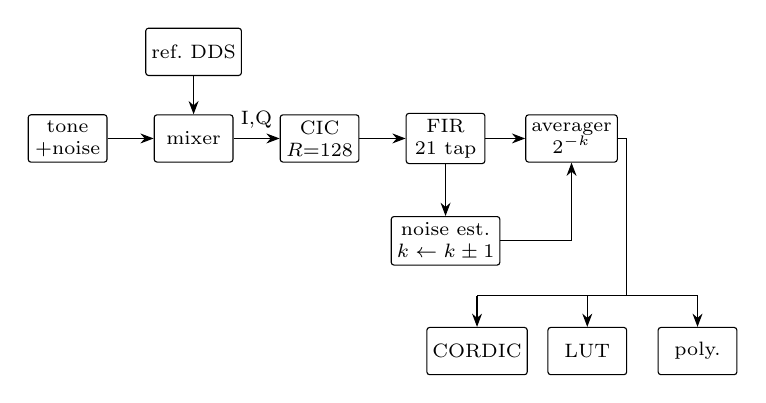
\begin{tikzpicture}[font=\scriptsize,>=Stealth,
 b/.style={draw,rounded corners=1pt,minimum height=0.6cm,minimum width=1.0cm,align=center,inner sep=2pt}]
 \node[b](src) at (0,0){tone\\+noise};
 \node[b](mix) at (1.6,0){mixer};
 \node[b](cic) at (3.2,0){CIC\\$R{=}128$};
 \node[b](fir) at (4.8,0){FIR\\21 tap};
 \node[b](avg) at (6.4,0){averager\\$2^{-k}$};
 \node[b](dds) at (1.6,1.1){ref.\ DDS};
 \node[b](ctl) at (4.8,-1.3){noise est.\\$k\leftarrow k\pm1$};
 \node[b](cor) at (5.2,-2.7){CORDIC};
 \node[b](lut) at (6.6,-2.7){LUT};
 \node[b](pol) at (8.0,-2.7){poly.};
 \draw[->](src)--(mix);
 \draw[->](mix)--node[above]{I,Q}(cic);
 \draw[->](cic)--(fir);
 \draw[->](fir)--(avg);
 \draw[->](dds)--(mix);
 \draw[->](fir.south)--(ctl.north);
 \draw[->](ctl.east)-|(avg.south);
 \draw(avg.east)--(7.1,0)--(7.1,-2.0);
 \draw(5.2,-2.0)--(8.0,-2.0);
 \draw[->](5.2,-2.0)--(cor.north);
 \draw[->](6.6,-2.0)--(lut.north);
 \draw[->](8.0,-2.0)--(pol.north);
\end{tikzpicture}}
\caption{Lock-in data path inside \texttt{lockin\_top}. The three extractors read the same averaged I/Q. The controller sets the averaging exponent $k$.}
\label{fig:arch}
\end{figure}

\subsection{Reference, stimulus and mixer}
The reference is a 32-bit phase accumulator addressing a 1024-entry sine ROM (the top 10 bits). The stimulus for the on-board experiments is generated in the same block: a second accumulator gives $A\cos(\omega_s n+\phi)$ in Q3.13, and noise is formed from four 16-bit slices of two xorshift32 generators, summed (variance of four uniforms) and scaled by $\sigma$ so that the standard deviation is $\sigma$ LSB. The sum of four uniform variables is close to Gaussian but not identical; measured kurtosis is 2.70 against 3 for a Gaussian. The sample is
\begin{equation}
x[n]=\operatorname{sat}_{16}\!\big(A\cos(\theta_s[n])+\sigma\,\nu[n]\big),
\end{equation}
and the mixer outputs $m_I[n]=x[n]\cos\theta_r[n]$ and $m_Q[n]=-x[n]\sin\theta_r[n]$, each a Q4.28 product that is rounded and saturated to 16 bits.

\subsection{CIC and FIR}
Each channel has a 4-stage CIC decimator with $R=128$ followed by a 21-tap compensating FIR. At a nominal sample rate of 200\,kS/s\nom{} this gives $200\,000/128=1562.5$ outputs per second (one every 0.64\,ms).

\subsection{Adaptive averaging}\label{sec:adapt}
The FIR outputs $y_I,y_Q$ are averaged by a first-order recursive filter with gain $2^{-k}$:
\begin{equation}
z[m]=z[m-1]+2^{-k}\,(y[m]-z[m-1]),\qquad k\in[0,20],
\end{equation}
held in 40-bit registers with 22 fractional bits. After a warm-up of 128 outputs (64 skipped, then two blocks of 32), the controller keeps a running estimate $\hat v$ of the variance of the FIR output about its mean. Every 32 outputs it estimates the signal power $\hat S=|\bar z|^2-2\hat v$ (clipped at zero) and updates
\begin{equation}
k\leftarrow\begin{cases}k+1,&\hat v>\hat S/2^{7}\\ k-1,&\hat v<\hat S/2^{9}\\ k,&\text{otherwise,}\end{cases}
\end{equation}
which is a dead-band controller on the ratio of noise variance to signal power. If the noise is large relative to the signal the filter narrows; if it is small the filter widens (shorter settling time). An anti-windup clamp keeps $k$ no larger than the number of blocks already averaged. The thresholds $2^{-7}$ and $2^{-9}$ were chosen by simulation so that the relative error of $|z|$ stays at a few percent; they are fixed in the hardware and are not tuned per run. In fixed mode, $k$ is set from a register.

The settling time of this filter to 10\,\% of a step is $\ln(10)\,2^k$ output periods, i.e.\ $1.47\,\mathrm{ms}\times2^k$ at the nominal rate. For $k=4,8,12$ this is $23.6$\,ms, $377$\,ms and $6.0$\,s.

\subsection{Magnitude and phase extraction}
The averaged $(\bar I,\bar Q)$ is passed to three extractors that run on the same input:
\begin{itemize}
\item \textbf{CORDIC}: 16 vectoring iterations, 16-bit data, with gain compensation. A guard-bit option exists in the C model (3 guard bits) and is evaluated there only.
\item \textbf{LUT}: 256-entry arctangent and magnitude tables with linear interpolation.
\item \textbf{Polynomial}: Horner evaluation of an order-5 arctangent polynomial and an order-3 magnitude-scale polynomial, with 16-bit saturating accumulators.
\end{itemize}
Angles are $\theta=\operatorname{atan2}(\bar Q,\bar I)$, stored in degrees as Q10.6 (CORDIC, LUT) or in units of $1/256^\circ$ (polynomial).

\section{Implementation on the PYNQ-ZU}
\subsection{Tool flow}
The design is written in C++ with Vitis HLS 2023.1, exported as an IP core, and integrated in Vivado 2023.1 with a JTAG-to-AXI master, an AXI interconnect, a clock wizard (100\,MHz) and a processor-system reset. The target is the XCZU5EG-SFVC784-1-E on the PYNQ-ZU. Two builds of the block design exist. The first has only the JTAG-to-AXI master; all experiments in Sections V-VI except the ARM runs use it, so those results do not depend on Linux. The second adds the Zynq UltraScale+ processing system as a second AXI master (HPM0\_FPD, 128 to 32-bit width converter in the interconnect), keeping the same 100\,MHz fabric clock from the board oscillator, and places the IP at 0xA0000000 for both masters. This second build is controlled from Python on the PYNQ 3.1.1 Linux image running on the Cortex-A53.

\subsection{Interface}
All parameters and results are AXI4-Lite registers (Table~\ref{tab:regs}). The block runs by writing \texttt{0x81} to the control register (start and auto-restart), after which it executes one sample per invocation continuously. A 512-record log memory (16 words per record) is read back through the same bus.
\begin{table}[t]\centering\caption{Selected AXI4-Lite registers (base 0x40000000)}\label{tab:regs}
\begin{tabular}{@{}llp{1.55in}@{}}\toprule
Offset & Name & Meaning\\\midrule
0x00 & ap\_ctrl & start / auto-restart\\
0x10 & ctl & reset, adaptive, log enable, ext.\ input, log clear\\
0x18 & kfix & fixed averaging exponent\\
0x20/28/30 & ph\_ref/ph\_sig/ph\_off & phase steps and offset\\
0x38/0x40 & amp, sigma & stimulus amplitude, noise $\sigma$\\
0x60 & out\_count & decimated outputs so far\\
0x90 & k\_now & current $k$\\
0x8000 & log\_mem & 8192 words\\\bottomrule
\end{tabular}\end{table}

\subsection{Code excerpts}
The two parts that carry the new function are the controller update and the call of the three extractors on the same averaged I/Q (from \texttt{ctrl\_x.cpp} and \texttt{lockin\_top.cpp}):
\begin{lstlisting}[language=C++]
if (adapt) {
  if (vm16 > (sig >> 7) && st.k < KMAX)      st.k = st.k + 1;
  else if (vm16 < (sig >> 9) && st.k > KMIN) st.k = st.k - 1;
}
...
cordic_vectoring(xi, xq, cm, ca);
lut_vectoring   (xi, xq, lm, la);
poly_vectoring  (xi, xq, pm, pa);
\end{lstlisting}
The top function uses one \texttt{s\_axilite} bundle for every port, including the log array. HLS reported an estimated maximum frequency of 137.2\,MHz. The requested \texttt{PIPELINE II=500} (to match 200\,kS/s) could not be applied (``unable to pipeline''), so the block finishes each sample in about 13--89 cycles and runs faster than the nominal 200\,kS/s. All time axes in this report are therefore labelled with the nominal rate\nom{}; the settling times in ms are in nominal time, and the ratios between settings are independent of the actual rate. The throughput measured on the board is 4.27\,MS/s (167\,332 decimated outputs in 5.015\,s, i.e.\ 33.4\,k outputs/s), 21.4 times the nominal rate, consistent with the HLS latency of 13--89 cycles at 100\,MHz. Real-time settling is therefore about 21 times shorter than the nominal times quoted below. The count was read over JTAG, so the interval has an uncertainty of a few milliseconds.

\section{Verification}
\subsection{Reference model and testbench}
A C reference (\texttt{ref\_pipe.c}) reproduces every stage with the same integer arithmetic. The HLS testbench runs the top function and the reference in lockstep over many configurations (fixed and adaptive modes, external input, reset and log-clear behaviour, and different amplitudes, noise levels and phase settings) and compares every logged word.
\subsection{Mutation testing}
To check that the testbench can actually fail, 17 single-line faults were injected one at a time into the source (for example: changed noise constant, inverted adaptive flag, swapped I/Q log words, removed anti-windup, an off-by-one in the log interval, wrong log-full flag). The testbench detected 17 of 17.
\subsection{On-board bit-exactness}
Seven configurations (V1--V7) were run on the FPGA; the full 512-record log (8192 words) of each was read back and compared word by word against the C model. All 57\,344 words match.
\subsection{ARM-controlled verification}
The same seven configurations were repeated on the processor build, this time started from Python on the Cortex-A53 (memory-mapped register access) and read back from the log memory. All 57\,344 words again match the C model. The JTAG route on the same bitstream gave the same result. Throughput measured from the ARM (167\,021 outputs in 5.005\,s, 4.2714\,MS/s) agrees with the JTAG measurement (4.271\,MS/s). A live run from Python with the amplitude fixed at 256 LSB and $\sigma$ stepped through 100, 1000, 3000, 8000, 1000, 100 showed $k$ settling at 0, 5, 8, 18--19, then back to 5 and 0 while the estimated magnitude stayed near the true value of 128.
\subsection{Reference sources and scope of the comparison}
The golden models were checked against independent numerical references, not only against themselves: the magnitude and angle extractors against NumPy \texttt{hypot} and \texttt{arctan2}, the FIR stage against SciPy \texttt{lfilter}, and the CIC stage against a direct convolution with the equivalent boxcar$^4$ response followed by decimation. The HLS blocks were then compared with these models using golden vectors (full-range and corner-case files for each extractor, plus mixer, DDS, chain and controller streams) in C simulation and Verilog co-simulation. The corner-case files cover the origin, all four axes, diagonal points, the extreme values $\pm32768$/$32767$, very small inputs and a set of points in each quadrant. No comparison against vendor IP (the Xilinx CIC and FIR compilers), MATLAB, or published test vectors was made.
\subsection{Extractor accuracy}
Extractor error was measured on the board for 4\,608 points, and over 4\,000\,256 inputs in the bit-accurate C model grouped by magnitude (powers of two).

\section{Results}
\subsection{Resources, timing and power}
Table~\ref{tab:res} gives post-implementation utilization (routed design) from the hierarchical report. The XCZU5EG has 117\,120 LUTs, 234\,240 flip-flops, 144 RAMB36 and 1\,248 DSP slices (device data sheet figures).
\begin{table}[t]\centering\caption{Post-implementation utilization of the lock-in IP (hierarchical report)}\label{tab:res}
\begin{tabular}{@{}lrrrr@{}}\toprule
Block & LUT & FF & DSP & BRAM\\\midrule
Adaptive controller & 3\,125 & 1\,815 & 6 & 0\\
Polynomial extractor & 1\,468 & 1\,368 & 9 & 0\\
LUT extractor & 1\,438 & 1\,351 & 3 & 2$^{c}$\\
CORDIC extractor & 776 & 218 & 1 & 0\\
FIR (I and Q, each) & 221--223 & 798 & 19 & 0\\
AXI-Lite slave & 667 & 420 & 0 & 8$^{a}$\\\midrule
Whole IP & 9\,554 & 12\,989 & 63 & 8+3$^{b}$\\
Whole design & 11\,008 & 15\,653 & 63 & 10+4$^{b}$\\\bottomrule
\end{tabular}\\[2pt]
{\scriptsize $^{a}$ RAMB36, holds the log memory. $^{b}$ RAMB36 + RAMB18; whole design includes the JTAG-AXI master. $^{c}$ Two RAMB18 holding the arctangent and magnitude tables. Per-block figures are measured inside the integrated IP and therefore differ slightly from the stand-alone HLS runs of the same blocks (for example CORDIC 668 LUT and polynomial 1\,528 LUT stand-alone).}
\end{table}
The IP uses 8.2\,\% of the LUTs and 5.0\,\% of the DSP slices. The 100\,MHz clock is met with worst setup slack $+3.256$\,ns and worst hold slack $+0.010$\,ns, with no failing endpoints. Vivado's vectorless power estimate for the whole design is 0.540\,W (0.220\,W dynamic, 0.319\,W static; junction 26.3\,$^\circ$C). Because the estimate is vectorless it is an indication, not a measurement.

Adding the processing system to the block design gives 12\,545 LUTs, 17\,319 flip-flops and 12 block RAM tiles for the whole design, still with the 100\,MHz clock met (setup slack $+3.551$\,ns, hold slack $+0.010$\,ns). The increase over the JTAG-only build is the AXI interface and width converter. The 2.8\,W power estimate of Vivado for this build is dominated by a default-configured processing system and is not a property of the lock-in IP, so the 0.54\,W figure above (JTAG-only build) is the one that applies to the IP.

\subsection{Comparison with the Cortex-A53}
To compare with software, the same \texttt{lockin\_top} C++ source was compiled with \texttt{g++ -O2} on the board's Cortex-A53 and run on one core for $5\times10^6$ samples in adaptive mode (amplitude 8192, $\sigma=300$). It processed 0.185\,MS/s (27.0\,s). The fabric implementation measured 4.27\,MS/s, i.e.\ about 23 times faster. This compares one source in two places; the software uses HLS arbitrary-precision integer types and is not a hand-optimized (for example NEON) implementation, so the ratio is specific to this code and a tuned ARM implementation would narrow the gap.

\subsection{Extraction accuracy}
Table~\ref{tab:ex} lists magnitude errors in input LSB and angle errors for three input-magnitude bins, from the C model (4\,000\,256 inputs, \texttt{guard}\,=\,0, the configuration on the board). Fig.~\ref{fig:ex} shows the full sweep.
\begin{table}[t]\centering\caption{Extractor error vs.\ input magnitude (C model; mag.\ RMS in LSB, angle RMS/max in degrees)}\label{tab:ex}
\begin{tabular}{@{}llrrr@{}}\toprule
Method & $|z|$ bin & mag RMS & ang RMS & ang max\\\midrule
CORDIC & 16--32 & 4.40 & 2.165 & 7.01\\
CORDIC & 256--512 & 3.34 & 0.166 & 0.81\\
CORDIC & 2048--4096 & 2.72 & 0.028 & 0.12\\
LUT & 16--32 & 0.51 & 0.012 & 0.024\\
LUT & 256--512 & 0.58 & 0.011 & 0.026\\
LUT & 2048--4096 & 0.76 & 0.011 & 0.026\\
Poly & 16--32 & 0.51 & 0.005 & 0.014\\
Poly & 256--512 & 0.62 & 0.006 & 0.019\\
Poly & 2048--4096 & 1.07 & 0.006 & 0.019\\\bottomrule
\end{tabular}\end{table}
\begin{figure}[t]\centering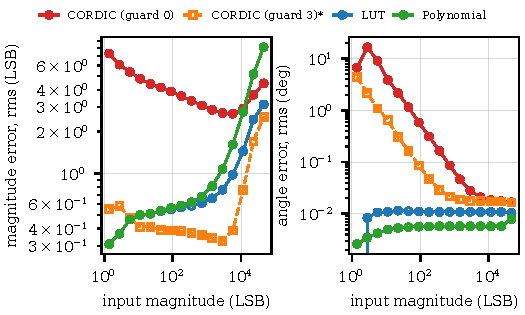
\includegraphics[width=\columnwidth]{fig/extract_err.pdf}
\caption{Extractor error against input magnitude.}\label{fig:ex}\end{figure}
With the default CORDIC (no guard bits) the magnitude carries a nearly constant bias of several LSB, which dominates for small inputs; the angle error is also largest there. A 3-guard-bit variant in the C model reduces the magnitude RMS to 0.33--0.58 LSB in the same bins, comparable to the LUT, but this variant has \emph{not} been run on the board. The LUT and polynomial methods have better angle accuracy than the unguarded CORDIC at every magnitude tested, and at the cost of more LUTs and DSP blocks (Table~\ref{tab:res}).

\subsection{Steady-state error of fixed and adaptive bandwidth}
For each noise level $\sigma$ the lock-in ran in fixed mode ($k=4,6,8,10,12$) and in adaptive mode, at input amplitudes of 1024 and 256 LSB, and the standard deviation of $|\bar I+j\bar Q|$ over the last 128 log records was divided by the true value $A/2$ (a fluctuation measure; it does not include bias) (Table~\ref{tab:s4}, Fig.~\ref{fig:noise}).
\begin{table}[t]\centering\caption{Relative fluctuation of $|\bar z|$ on the board (std.\ over the last 128 log records divided by the true value $A/2$, in \%); adaptive mean $k$ in brackets}\label{tab:s4}
\begin{tabular}{@{}rrrrrrr@{}}\toprule
$\sigma$ & $k{=}4$ & 6 & 8 & 10 & 12 & adaptive\\\midrule
\multicolumn{7}{@{}l}{\emph{amplitude 1024 LSB}}\\
100 & 0.2 & 0.1 & 0.0 & 0.0 & 0.0 & 1.1 (0)\\
300 & 0.7 & 0.3 & 0.1 & 0.1 & 0.0 & 3.2 (0)\\
1000 & 2.2 & 1.1 & 0.4 & 0.2 & 0.1 & 6.7 (1)\\
3000 & 6.6 & 3.2 & 1.3 & 0.5 & 0.2 & 6.6 (4)\\
8000 & 17.7 & 8.5 & 3.6 & 1.4 & 0.5 & 5.7 (7)\\\midrule
\multicolumn{7}{@{}l}{\emph{amplitude 256 LSB}}\\
100 & 0.9 & 0.4 & 0.2 & 0.1 & 0.0 & 4.3 (0)\\
300 & 2.6 & 1.3 & 0.5 & 0.2 & 0.1 & 5.6 (2)\\
1000 & 8.8 & 4.2 & 1.8 & 0.7 & 0.2 & 6.1 (5)\\
3000 & 26.5 & 12.8 & 5.4 & 2.1 & 0.7 & 5.4 (8)\\
8000 & 62.3 & 34.1 & 14.7 & 5.8 & 1.9 & 3.7 (11)\\\bottomrule
\end{tabular}\end{table}
\begin{figure}[t]\centering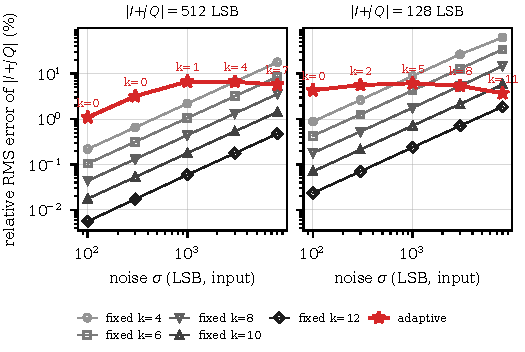
\includegraphics[width=\columnwidth]{fig/noise_sweep.pdf}
\caption{Relative error against noise for fixed $k$ and adaptive mode. Annotations: adaptive $k$.}\label{fig:noise}\end{figure}
The adaptive controller does not minimize the error; it holds it at a few percent (1.1--6.7\,\% in all ten cases) with the \emph{least} averaging that does so. At low noise and strong signal it stays at $k=0$ and responds immediately, while at the weakest signal and highest noise it raises $k$ to 11 and the error falls to 3.7\,\%, where fixed $k=4$ reaches 62.3\,\%. A fixed wide filter ($k\ge10$) gives lower error almost everywhere but with settling times of seconds. When the signal is strong and the noise low, adaptive mode is \emph{worse} than a fixed wide filter (for example 3.2\,\% against 0.1\,\% at $\sigma=300$, amplitude 1024), which is the price of the dead-band.

\subsection{Step responses}
In the amplitude-step experiment the amplitude drops from 512 to 64 LSB at $\sigma=300$. The 90\,\% settling time, measured on the board, is 20.5\,ms, 368.6\,ms and 6.02\,s for fixed $k=4$, 8 and 12 (nominal time), against the theoretical 23.6\,ms, 377\,ms and 6.0\,s. The adaptive mode, which is at $k=0$ before the step at high SNR, is within 10\,\% of the new value at the first log record after the step (log interval 20.5\,ms), and then raises $k$ to 4 as the SNR falls (Figs.~\ref{fig:step},\ref{fig:settle}). The step instant is known only to within the log interval, so the adaptive settling time is bounded by 20.5\,ms and not measured more finely.
\begin{figure}[t]\centering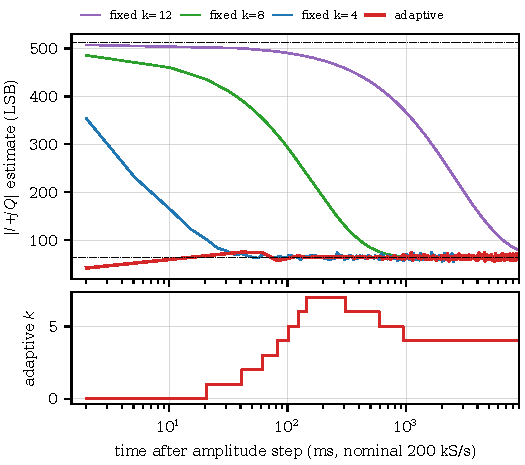
\includegraphics[width=\columnwidth]{fig/step_amp.pdf}
\caption{Amplitude step 512$\to$64 LSB: estimate and adaptive $k$ (nominal time).}\label{fig:step}\end{figure}
\begin{figure}[t]\centering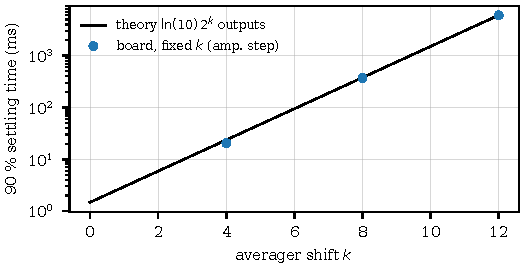
\includegraphics[width=\columnwidth]{fig/settle_k.pdf}
\caption{90\,\% settling time against $k$: theory and board.}\label{fig:settle}\end{figure}

\subsection{Weak-signal operation}
To test the regime in which a lock-in is normally needed, the amplitude was lowered to 64, 32, 16 and 8 LSB at $\sigma=8000$\,LSB, giving broadband input SNRs of $-45$, $-51$, $-57$ and $-63$\,dB ($\mathrm{SNR}=A^2/2\sigma^2$). Each run lasted about 90\,s of real time (512 log records, spacing 5\,865 outputs). The error is the RMS difference of $|\bar z|$ from the true $A/2$ over the last 128 records (Table~\ref{tab:deep}, Fig.~\ref{fig:deep}).
\begin{table}[t]\centering\caption{RMS error of $|\bar z|$ against the true value (\%), $\sigma=8000$ LSB; adaptive final $k$ in brackets}\label{tab:deep}
\begin{tabular}{@{}rrrrrr@{}}\toprule
SNR (dB) & $k{=}8$ & $k{=}12$ & $k{=}16$ & adaptive\\\midrule
$-45$ ($A{=}64$) & 57.3 & 17.0 & 2.8 & 4.4 (15)\\
$-51$ ($A{=}32$) & 119.5 & 33.8 & 5.6 & 4.2 (17)\\
$-57$ ($A{=}16$) & 280.8 & 65.3 & 11.4 & 5.7 (19)\\
$-63$ ($A{=}8$) & -- & -- & -- & 5.7 / 4.2 (20)$^{c}$\\\bottomrule
\end{tabular}\\[2pt]{\scriptsize $^{c}$ Two seeds; $k$ reached its limit of 20.}
\end{table}
\begin{figure}[t]\centering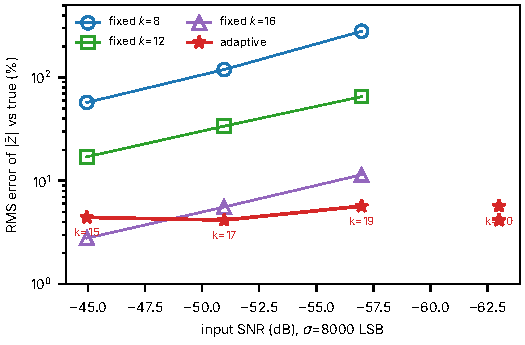
\includegraphics[width=\columnwidth]{fig/deep_noise.pdf}
\caption{Error against input SNR; adaptive $k$ annotated.}\label{fig:deep}\end{figure}
Without any setting by the user, the adaptive mode chose $k=15,17,19,20$ and held 4--6\,\% error, whereas fixed $k=8$ and 12 fail at these SNRs. A well-chosen fixed $k=16$ is better at $-45$\,dB (2.8\,\%) but needs a wrong guess of $k$ to be right in advance, and at $-57$\,dB gives 11.4\,\%. At $-63$\,dB the controller has reached its upper limit ($k=20$, time constant $2^{20}$ outputs, about 31\,s of board time), and only two seeds were run, so the error figures there are indicative. The magnitude estimate is biased upward when the averaged noise is comparable to the signal (a fixed $k=8$ reads 26 instead of 8 at $-57$\,dB); this is why the errors above are measured against the true value and not against the spread alone. The consecutive records are correlated at large $k$ because the filter time constant exceeds the record spacing, so the spread within a run understates the run-to-run variation.

\section{Limitations}
\begin{itemize}
\item The on-board input is synthetic (internal tone plus pseudo-random noise); no ADC, analog front end, or function generator was used. The noise is close to Gaussian but not exact.
\item The pipelining directive for 200\,kS/s was not honoured, so the block is not paced to 200\,kS/s; times in ms in the step-response figures are nominal\nom{}. Throughput was measured once (4.27\,MS/s) over JTAG polling, not with an external time base.
\item Power is a vectorless estimate for the JTAG-only build. The processor build has not been given its own power figure.
\item The A53 comparison uses the HLS source unchanged on one core; it is not an optimized ARM implementation.
\item The equilibrium of $k$ depends on history: in the live run $k$ reached 18--19 at $\sigma=8000$ and amplitude 256, higher than the mean of 11 in the logged cold-start run at the same settings, and it fell back only after the noise was reduced. This is consistent with the hysteresis between the $2^{-7}$ and $2^{-9}$ thresholds but was not investigated further, and an upward noise step can leave $k$ higher than needed for several seconds.
\item The adaptive thresholds are fixed constants chosen by simulation; no optimality is claimed, and a comparison with a Kalman-filter DLIA \cite{chen} was not made.
\item The 3-guard-bit CORDIC is evaluated in the C model only.
\item The saturation branch of the polynomial evaluator was not triggered by any test vector, and the corner-case vectors were not chosen to hit the lookup-table breakpoints specifically, so those two paths have less direct coverage than the rest.
\item The adaptive results are for stationary signals and single noise or amplitude steps.
\end{itemize}

\section{Conclusion}
A streaming DLIA with online-SNR bandwidth selection and three interchangeable extractors was implemented on an XCZU5EG, reproduced bit-exactly on the board, and measured against fixed-bandwidth operation. The routed design uses under 10\,\% of the device and meets 100\,MHz timing. The adaptive rule keeps the amplitude error at 1--7\,\% across an 80:1 noise range and down to $-63$\,dB input SNR with the least averaging that achieves it, at the cost of a higher error than a wide fixed filter when the signal is strong, and the extractor study shows the accuracy/area trade-off among CORDIC, LUT and polynomial methods. Natural next steps are a real ADC input, an external-time-base throughput measurement, and a tuned or learned adaptation rule.

\nom{} Nominal rate; see Section~IV.

\begin{thebibliography}{10}
\bibitem{fan} S. X. Fan, Z. A. He, L. H. Xing, N. Chen, and D. P. Fan, ``Design of digital lock-in amplifier based on ZYNQ-7020,'' in \emph{Proc.\ CSAA/IET Int.\ Conf.\ Aircraft Utility Systems (AUS 2022)}, Nanchang, China, Aug.\ 17--20, 2022, pp.~1428--1433, doi: 10.1049/icp.2022.1881.
\bibitem{zhang} C. Zhang, H. Liu, J. Ge, and H. Dong, ``FPGA-based digital lock-in amplifier with high-precision automatic frequency tracking,'' \emph{IEEE Access}, vol.~8, pp.~123114--123122, Jun.\ 30, 2020, doi: 10.1109/ACCESS.2020.3006070.
\bibitem{yao} Z. Yao, J. Pan, C. Yu, Z. Yuan, Q. Chen, and X. Sui, ``A universal digital lock-in amplifier design for calibrating the photo-detector responses with standard black-bodies,'' \emph{Sensors}, vol.~23, no.~21, p.~8902, Nov.\ 1, 2023, doi: 10.3390/s23218902.
\bibitem{olia} A. J. Harvie and J. C. de Mello, ``OLIA: An open-source digital lock-in amplifier,'' \emph{Front.\ Sens.}, vol.~4, art.\ 1102176, Mar.\ 30, 2023, doi: 10.3389/fsens.2023.1102176.
\bibitem{chen} H. Chen, Y. Li, and L. Ou, ``A digital lock-in amplifier based on adaptive Kalman filter for rail defect detection,'' \emph{J.\ Sensors}, vol.~2023, art.\ 7112942, 11~pp., 2023, doi: 10.1155/2023/7112942.
\bibitem{acfm} J. Ge, X. Chen, and B. Hu, ``Development of a velocity-adaptable alternating current field measurement device for crack inspection in rails,'' \emph{IEEE Sensors J.}, vol.~23, no.~15, pp.~17034--17041, Aug.~1, 2023.
\bibitem{volder} J. E. Volder, ``The CORDIC trigonometric computing technique,'' \emph{IRE Trans.\ Electron.\ Comput.}, vol.~EC-8, no.~3, pp.~330--334, 1959.
\bibitem{hogenauer} E. B. Hogenauer, ``An economical class of digital filters for decimation and interpolation,'' \emph{IEEE Trans.\ Acoust., Speech, Signal Process.}, vol.~29, no.~2, pp.~155--162, 1981.
\end{thebibliography}
\end{document}
